\documentclass[professionalfonts]{beamer}
\newif\ifita
%\itatrue
\itafalse
\usepackage[familydefault,light]{Chivo} 
\usepackage[T1]{fontenc}
\usenavigationsymbolstemplate{}
\usepackage[]{hyperref}
\usepackage{tikz,pgf,pgfarrows,pgfnodes,pgfbaseimage}
\graphicspath{{./Pics/}}
\usetikzlibrary{shapes}
\usepackage{setspace}
\newcommand{\evi}[1]{{\colorbox{yellow!50}{{#1}}}}
\newcommand{\exe}[1]{{\color{black!50}{{#1}}}}
\newcommand{\kw}[1]{{\colorbox{black!30}{\color{white}{#1}}}}
\tikzstyle{nd}=[circle,draw=black,thick,minimum size=.8cm,inner sep=1pt]
\setbeamercovered{transparent}
\usetheme{Singapore}
\tikzstyle{nodo}=[ellipse,draw=black!60,fill=black!10,line width=.7pt,minimum width=.7cm,minimum height=.4cm]
\usecolortheme[named=gray]{structure}
\setbeamercolor{block title}{bg=black!20,fg=black}
\setbeamercolor{block body}{bg=black!10,fg=black}

\ifita
\title{Algoritmi Numerici (Parte II)}
\subtitle{[Lezione 3 \& 4] Algoritmi di Ricorsivi\\Metodi della Secante e Tangente}
\else
\title{Numerics (Part II)}
\subtitle{[Lectures 3 \& 4] Recursive Algorithms\\Secant and Tangent Methods}
\fi
\date{}
\author{Alessandro Antonucci\\{\tt alessandro.antonucci@supsi.ch}}
\begin{document}
\maketitle
\setstretch{1.4}
%\date{\tiny\url{https://colab.research.google.com/drive/1Iv2YA4iBL8g54yY1bdcRgtFNqI4LF7Kw}}
%%%%%%%%%%%%%%%%%%%%%%%%%%%%
\frame{\frametitle{\ifita Ricorsioni \else Recursions \fi}
\begin{itemize}
\ifita
\item Sequenza $x_0$, $x_1$, $x_2$, $\ldots$ generata da una ricorsione
\item (ex1) fattoriale $x_{j+1} = (j+1) x_j$ (con $x_0=1$)
\item (ex2) Fibonacci $x_{j+1} = x_j + x_{j-1}$ (con $x_0=1$ e $x_1=2$)
\item (ex1) ricorsione ordine 1,\\inizializzazione solo del primo elemento
\item (ex2) ricorsione ordine 2,\\inizializzazione dei primi due elementi
\else
\item Sequence $x_0$, $x_1$, $x_2$, $\ldots$ generated by recursion
\item (ex1) factorial $x_{j+1} = (j+1) x_j$ (where $x_0=1$)
\item (ex2) Fibonacci $x_{j+1} = x_j + x_{j-1}$ (where $x_0=1$ e $x_1=2$)
\item (ex1) 1st order recursion,\\initializing only the first element
\item (ex2) 2nd order recursion,\\initializing the first two elements
\fi
\end{itemize}}


\frame{\frametitle{Identificazione degli zeri mediante sequenze}
\begin{itemize}
\ifita
\item Approssimare zero $x^*$ di una funzione $f(x)$?
\item Sequenza $x_0$, $x_1$, $\ldots$, $x_n$ che si avvicina ad $x^*$
\item Convergenza: $\lim_{n\to+\infty} |x_n-x^*| = 0$
\else
\item Approximating zero $x^*$ of function $f(x)$?
\item Sequence $x_0$, $x_1$, $\ldots$, $x_n$ approaching $x^*$
\item Convergence: $\lim_{n\to+\infty} |x_n-x^*| = 0$
\fi
\end{itemize}
\begin{columns}
\begin{column}[T]{0.5\textwidth}
\begin{block}{\ifita SECANTE \else SECANT \fi}
\begin{center}
$x_{j+1} = x_j - \frac{f(x_j)}{ \frac{f(x_j)-f(x_{j-1})}{x_j-x_{j-1}}}$
\end{center}
\end{block}
\end{column}
\begin{column}[T]{0.5\textwidth}
\begin{block}{\ifita TANGENTE \else TANGENT \fi}
\begin{center}
$x_{j+1} = x_j - \frac{f(x_j)}{f'(x_j)}$
\end{center}
\end{block}
\end{column}
\end{columns}
\begin{center}
\ifita
\emph{Nota: nessuno dei due algoritmi garantisce convergenza}
\else
\emph{Note: none of the two algorithms guarantee convergence}
\fi
\end{center}}


\frame{\frametitle{\ifita Algoritmo della Secante \else Secant Algorithm\fi}
\setbeamercovered{}
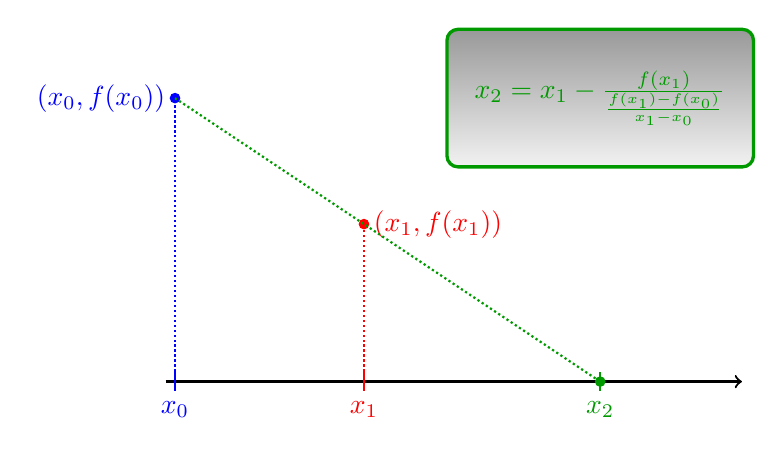
\begin{tikzpicture}[domain=0:3.5,scale=1.2]
\draw[->,thick] (-.1,0) -- (6,0);
\draw[thick,color=orange] plot[id=exp] function{3-x*x*1/3}; 
\pause
\draw[blue,thick] (0,.1) -- (0,-.1) node[below] {$x_0$};
\draw[red,thick] (2,.1) -- (2,-.1) node[below] {$x_1$};
\pause
\draw[blue,densely dotted,thick] (0,0) -- (0,3);
\draw [blue,fill] (0,3) circle [radius=0.05] node[left] {$(x_0,f(x_0))$};
\draw [red,fill] (2,5/3) circle [radius=0.05] node[right] {$(x_1,f(x_1))$};
\draw[densely dotted,red,thick] (2,0) -- (2,5/3);
\pause
\draw[densely dotted,green!60!black,thick] (0,3) -- (9/2,0);
\pause
\draw [green!60!black,fill] (9/2,0) circle [radius=0.05] node[right] {};
\draw[green!60!black,thick] (9/2,.1) -- (9/2,-.1) node[below] {$x_2$};
\draw[green!60!black,thick] (9/2,3) node[top color=black!40,bottom color=black!5,very thick,draw,rectangle, rounded corners, inner sep=10pt, inner ysep=15pt] {$x_2=x_1-\frac{f(x_1)}{\frac{f(x_1)-f(x_0)}{x_1-x_0}}$};
\end{tikzpicture}}


\frame{\frametitle{\ifita Algoritmo della Tangente \else Tangent Algorithm \fi}
\setbeamercovered{}
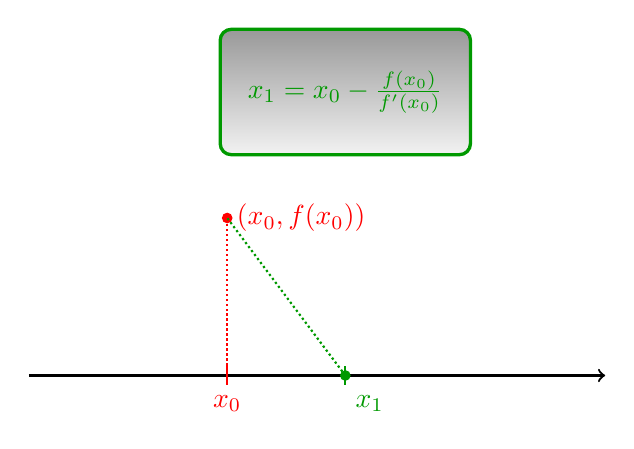
\begin{tikzpicture}[domain=0:3.5,scale=1.2]
\draw[->,thick] (-.1,0) -- (6,0);
\draw[thick,color=orange] plot[id=exp] function{3-x*x*1/3}; 
\pause
\draw[red,thick] (2,.1) -- (2,-.1) node[below] {$x_0$};
\pause
\draw [red,fill] (2,5/3) circle [radius=0.05] node[right] {$(x_0,f(x_0))$};
\draw[densely dotted,red,thick] (2,0) -- (2,5/3);
\pause
\draw[densely dotted,green!60!black,thick] (13/4,0) -- (2,5/3);
\pause
\draw [green!60!black,fill] (13/4,0) circle [radius=0.05] node[right] {};
\draw[green!60!black,thick] (13/4,.1) -- (13/4,-.1) node[below right] {$x_1$};
\draw[green!60!black,thick] (13/4,3) node[top color=black!40,bottom color=black!5,very thick,draw,rectangle, rounded corners, inner sep=10pt, inner ysep=15pt] {$x_1=x_0-\frac{f(x_0)}{f'(x_0)}$};
\end{tikzpicture}}


\frame{\frametitle{\ifita Algoritmo della Secante\else Secant Algorithm \fi}
\setbeamercovered{}
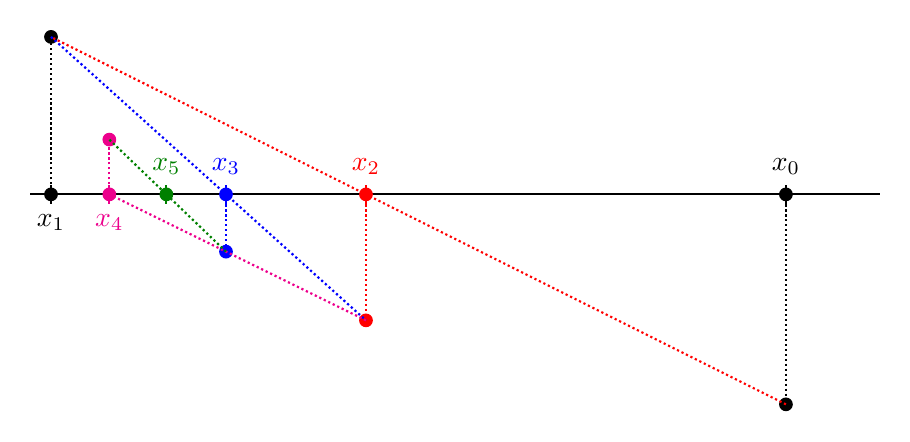
\begin{tikzpicture}[domain=0.5:3.3,scale=4]
\draw[-,thick] (0.6,0) -- (3.3,0);
\draw[thick,color=black] plot[id=exp] function{1/x-1}; 
\pause
\draw[black,thick] (3,-.03) -- (3,.03) node[above] {$x_0$};
\draw[black,thick] (2/3,.03) -- (2/3,-.03) node[below] {$x_1$};
\draw [black,fill] (3,0) circle [radius=0.02] node[left] {};
\draw [black,fill] (2/3,0) circle [radius=0.02] node[right] {};
\pause
\draw[black,densely dotted,thick] (3,0) -- (3,-2/3);
\draw[black,densely dotted,thick] (2/3,0) -- (2/3,1/2);
\draw [black,fill] (3,-2/3) circle [radius=0.02] node[left] {};
\draw [black,fill] (2/3,1/2) circle [radius=0.02] node[right] {};
\pause
\draw[densely dotted,thick,red] (3,-2/3) -- (2/3,1/2);
\pause
\draw [red,fill] (5/3,0) circle [radius=0.02] node[right] {};
\draw[red,thick] (5/3,-.03) -- (5/3,.03) node[above] {$x_2$};
\pause
\draw[densely dotted,thick,red] (5/3,0) -- (5/3,-2/5);
\draw [red,fill] (5/3,-2/5) circle [radius=0.02] node[right] {};
\pause
\draw[densely dotted,thick,blue] (2/3,1/2) -- (5/3,-2/5);
\pause
\draw [blue,fill] (11/9,0) circle [radius=0.02] node[right] {};
\draw[blue,thick] (11/9,-.03) -- (11/9,.03) node[above] {$x_3$};
\pause
\draw[densely dotted,thick,blue] (11/9,0) -- (11/9,-2/11);
\draw [blue,fill] (11/9,-2/11) circle [radius=0.02] node[right] {};
\pause
\draw[densely dotted,thick,magenta] (5/3,-2/5) -- (23/27,0);
\pause
\draw [magenta,fill] (23/27,0) circle [radius=0.02] node[right] {};
\draw[magenta,thick] (23/27,.03) -- (23/27,-.03) node[below] {$x_4$};
\pause
\draw[densely dotted,thick,magenta] (23/27,0) -- (23/27,4/23);
\draw [magenta,fill] (23/27,4/23) circle [radius=0.02] node[right] {};
\pause
\draw[densely dotted,thick,green!50!black] (11/9,-2/11) -- (23/27,4/23);
\pause
\draw [green!50!black,fill] (251/243,0) circle [radius=0.02] node[right] {};
\draw[green!50!black,thick] (251/243,-.03) -- (251/243,.03) node[above] {$x_5$};
\end{tikzpicture}}




\frame{\frametitle{\ifita Algoritmo della Tangente\else Tangent Algorithm \fi}
    \setbeamercovered{}
    \begin{tikzpicture}[domain=0.5:3.3,scale=1]
        %\draw[-,thick] (0.6,0) -- (3.3,0);
        \draw[thick,color=black] plot[id=exp2] function{x*x-1}; 
%        \pause
%        \draw[black,thick] (3,-.03) -- (3,.03) node[above] {$x_0$};
%        \draw[black,thick] (2/3,.03) -- (2/3,-.03) node[below] {$x_1$};
%        \draw [black,fill] (3,0) circle [radius=0.02] node[left] {};
%        \draw [black,fill] (2/3,0) circle [radius=0.02] node[right] {};
%        \pause
%        \draw[black,densely dotted,thick] (3,0) -- (3,-2/3);
%        \draw[black,densely dotted,thick] (2/3,0) -- (2/3,1/2);
%        \draw [black,fill] (3,-2/3) circle [radius=0.02] node[left] {};
%        \draw [black,fill] (2/3,1/2) circle [radius=0.02] node[right] {};
%        \pause
%        \draw[densely dotted,thick,red] (3,-2/3) -- (2/3,1/2);
%        \pause
%        \draw [red,fill] (5/3,0) circle [radius=0.02] node[right] {};
%        \draw[red,thick] (5/3,-.03) -- (5/3,.03) node[above] {$x_2$};
%        \pause
%        \draw[densely dotted,thick,red] (5/3,0) -- (5/3,-2/5);
%        \draw [red,fill] (5/3,-2/5) circle [radius=0.02] node[right] {};
%        \pause
%        \draw[densely dotted,thick,blue] (2/3,1/2) -- (5/3,-2/5);
%        \pause
%        \draw [blue,fill] (11/9,0) circle [radius=0.02] node[right] {};
%        \draw[blue,thick] (11/9,-.03) -- (11/9,.03) node[above] {$x_3$};
%        \pause
%        \draw[densely dotted,thick,blue] (11/9,0) -- (11/9,-2/11);
%        \draw [blue,fill] (11/9,-2/11) circle [radius=0.02] node[right] {};
%        \pause
%        \draw[densely dotted,thick,magenta] (5/3,-2/5) -- (23/27,0);
%        \pause
%        \draw [magenta,fill] (23/27,0) circle [radius=0.02] node[right] {};
%        \draw[magenta,thick] (23/27,.03) -- (23/27,-.03) node[below] {$x_4$};
%        \pause
%        \draw[densely dotted,thick,magenta] (23/27,0) -- (23/27,4/23);
%        \draw [magenta,fill] (23/27,4/23) circle [radius=0.02] node[right] {};
%        \pause
%        \draw[densely dotted,thick,green!50!black] (11/9,-2/11) -- (23/27,4/23);
%        \pause
%        \draw [green!50!black,fill] (251/243,0) circle [radius=0.02] node[right] {};
%        \draw[green!50!black,thick] (251/243,-.03) -- (251/243,.03) node[above] {$x_5$};
\end{tikzpicture}}



\end{document}
